\documentclass[12pt]{article}

\usepackage[numbers]{natbib}
\usepackage{graphicx}
\usepackage{amsmath}
\usepackage{tikz}

\title{Temperature Control.}
\author{Alex Kleeman}

\begin{document}
\maketitle

Consider the case of some object which is being heated internally.  With constant volume, the change in temperature, $u$, of the body will change at a rate of,
\[
\frac{\partial u}{\partial t} = \frac{\dot{Q}}{C_V}.
\]
where $\dot{Q}$ is the rate at which heat is added in units of watts, $W$, and $C_V$ is the volumetric heat capacity in units of $\frac{J}{K}$.

There may be several sources of heat addition or loss.  Heat added from an external source may be a fixed term, $\dot{Q}_{ext}$, while heat lost from convection would take the form $h A (u - u_{env})$, where $h$ is the heat transfer coefficient and $A$ is the exposed area and $u_{env}$ is the temperature of the surroundings.

We can then model the change in temperature using the differential equation,
\[
\frac{\partial u}{\partial t} = \frac{\dot{Q}_{ext} + hA (u - u_{env})}{C_V}
\]

\begin{figure}[ht!]
\centering
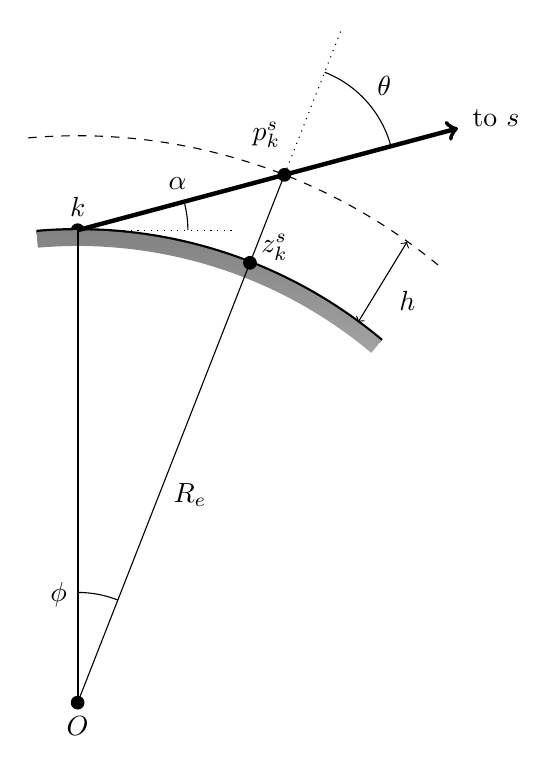
\begin{tikzpicture}[xscale=-1,
    ray/.style={decoration={markings,mark=at position .5 with {
      \arrow[>=latex]{>}}},postaction=decorate}
  ]

  % Radius of earth
  \pgfmathsetlengthmacro{\r}{6cm}
  % View Angle
  \pgfmathsetlengthmacro{\a}{40}
  \pgfmathsetlengthmacro{\aleft}{85}
  \pgfmathsetlengthmacro{\aright}{90+\a}
  % Height of the Ionosphere
  \pgfmathsetlengthmacro{\h}{1.2cm}
  % Elevation angle
  \pgfmathsetlengthmacro{\e}{15}
  % Line of sight length
  \pgfmathsetlengthmacro{\los}{5cm}

  \pgfmathsetlengthmacro{\pi}{3.141592653589}
  \pgfmathsetlengthmacro{\aphi}{90 - \e - asin(\r / (\r + \h) * sin(90 - \e))}
  \pgfmathsetlengthmacro{\atheta}{90 - (\aphi + \e)}
  % Various radii for drawing angle arcs and labels
  \pgfmathsetlengthmacro{\arcradius}{1.4cm}
  \pgfmathsetlengthmacro{\dotradius}{1.2cm}
  \pgfmathsetlengthmacro{\arclabelradius}{1.8cm}
  \pgfmathsetlengthmacro{\pointradius}{0.08cm}

  % Coordinates of origin
  \coordinate (O) at (0, 0);
  \draw (O) ++(270:0.3cm) node {$O$};
  \draw[fill] (O) circle (\pointradius);
  % Receiver
  \coordinate (R) at (0, \r);
  \draw (R) ++(90:0.3cm) node {$k$};
  \draw[fill] (R) circle (\pointradius);
 
  \draw (R) ++(180-\e:\los+0.5cm) node {to $s$};
  %\draw[fill] (R) ++(180-\e:\los) circle (\pointradius);

  % Draw the earth and the ionosphere
  \draw[ultra thick] (O) ++(\aleft:\r) arc[radius=\r, start angle=\aleft, end angle=\aright];
  \draw[dashed, thin] (O) ++(\aleft:\r+\h) arc (\aleft:\aright:\r + \h);

  \shade (0,0) ++(\aleft:\r-0.2cm) -- ++(\aleft:0.2cm) arc (\aleft:\aright:\r) -- ++(\aright+180:0.2cm) arc (\aright:\aleft:\r-0.2cm);

  % And the line to the center of the earth and a label
  \draw[thick] (O) -- (R);

  % Line tangent to the receiver
  \draw[dotted, thin] (R) -- ++(180:2);
  % Draw the Line of Sight to the Satellite
  \draw[->, ultra thick] (O) ++(90:\r) -- ++(180-\e:\los);
  \draw (R) ++(180:\arcradius) arc[radius=\arcradius, start angle=180, end angle=180-\e];
  \draw (R) ++(180-\e-10:\arcradius) node {$\alpha$};

  % Center of earth to pierce point
  \draw (O) -- ++(90+\aphi:\r + \h);
  \draw[fill] (O) ++(90+\aphi:\r + \h) circle (\pointradius);
  \draw (O) ++(87+\aphi:\r + \h + 0.4cm) node {$p_k^s$};
  % Projected Pierce Point
  \draw[fill] (O) ++(90+\aphi:\r) circle (\pointradius);
  \draw (O) ++(92+\aphi:\r+0.3cm) node {$z_k^s$};

  \draw (O) ++(90:\arcradius) arc[radius=\arcradius, start angle=90, end angle=90+\aphi];
  \draw (O) ++(80:\arcradius) node {$\phi$};

  % Radius labels
  \pgfmathsetlengthmacro{\halfr}{\r / 2};
  \draw (O) ++(97+\aphi:\halfr) node {$R_{e}$};
  \pgfmathsetlengthmacro{\halfh}{\h / 2};
  \draw[<->] (O) ++(105+\aphi:\r) -- ++(100+\aphi:\h);
  \draw (O) ++(108+\aphi:\r + \halfh) node {$h$};

  %Angle of Incidence
  \pgfmathsetlengthmacro{\halftheta}{\atheta / 2};
  \draw[dotted] (0, 0) ++(90+\aphi:\r + \h) -- ++(90+\aphi:2);
  \draw (O) ++(90+\aphi:\r + \h) ++(180-\e:\arcradius) arc[radius=\arcradius, start angle=180-\e, end angle=90+\aphi];
  \draw (O) ++(90+\aphi:\r + \h) ++(180-\e-\halftheta:\arcradius+0.3cm) node {$\theta$};


\end{tikzpicture}
\caption{The geometry that describes the pierce point, $p_k^s$, for a signal traveling from the receiver, $k$, to a satellite, $s$, with elevation angle $\alpha$ through a thin shell approximation of ionosphere with height $h$.  The diagram here shows a slice taken through the points $k$, $p_k^s$ and the center of the earth, $O$, which makes the arc length between $k$ and the surface projection of the pierce point, $z_k^s$, a great circle route with distance $R_{e} \Phi$.}
\label{fig:pierce}
\end{figure}

\end{document}


